\section{Conceitos iniciais}

\begin{frame}[allowframebreaks]{Conceitos iniciais}

\begin{itemize}
    \item Função: é uma regra ou lei que associa cada elemento de um conjunto um único elemento de outro conjunto.

    \vspace{0.5cm}

    \begin{multicols}{2}
        \begin{figure}
        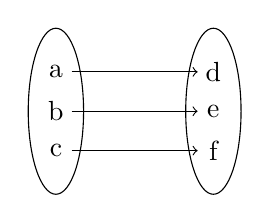
\begin{tikzpicture}
            \draw (0,0) ellipse (10pt and 30pt);
            \draw (2,0) ellipse (10pt and 30pt);

            \draw node at (0, 0.5) {a};
            \draw node at (0, 0) {b};
            \draw node at (0, -0.5) {c};

            \draw node at (2, 0.5) {d};
            \draw node at (2, 0) {e};
            \draw node at (2, -0.5) {f};

            \draw [->] (0 + 0.2, 0.5) -- (2 - 0.2, 0.5);
            \draw [->] (0 + 0.2, 0) -- (2 - 0.2, 0);
            \draw [->] (0 + 0.2, -0.5) -- (2 - 0.2, -0.5);
    \end{tikzpicture}
    \caption{É função}
    \end{figure}

    \begin{figure}
        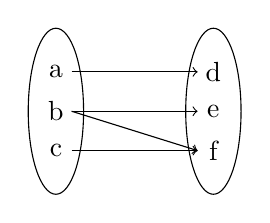
\begin{tikzpicture}
            \draw (0,0) ellipse (10pt and 30pt);
            \draw (2,0) ellipse (10pt and 30pt);

            \draw node at (0, 0.5) {a};
            \draw node at (0, 0) {b};
            \draw node at (0, -0.5) {c};

            \draw node at (2, 0.5) {d};
            \draw node at (2, 0) {e};
            \draw node at (2, -0.5) {f};

            \draw [->] (0 + 0.2, 0.5) -- (2 - 0.2, 0.5);
            \draw [->] (0 + 0.2, 0) -- (2 - 0.2, 0);
            \draw [->] (0 + 0.2, 0) -- (2 - 0.2, -0.5);
            \draw [->] (0 + 0.2, -0.5) -- (2 - 0.2, -0.5);
    \end{tikzpicture}
    \caption{Não é função}
    \end{figure}
    \end{multicols}

    \skipframe

    \item De forma prática, pode-se ver, através de um gráfico, se uma relação é uma função pelo \emph{teste da reta vertical}.

    \item O teste consiste em traçar retas verticais por pontos do eixo $x$ (domínio) e, se ela cortar o gráfico em mais de um ponto, esta relação não representa uma função.

    \skipframe

    \begin{figure}
        \centering
        \begin{tikzpicture}[scale=0.8]
        \draw[color=blue] (3.43,2.85) circle (1);
        \draw[color=red] (2.8, 5) -- (2.8, 1);
        \begin{axis}[xmin=-5, xmax=5, ymin=-5, ymax=5, axis lines=middle]
        \end{axis}
        \end{tikzpicture}
        \caption{Não é função}
    \end{figure}

    \skipframe

    \item O método mais comum de visualizar uma função consiste em fazer seu gráfico. 

    \item Dada uma função $f:A \rightarrow B$, o gráfico de $f$ será o conjunto de pares ordenados $G(f) = \conj{(x, f(x)) \mid x \in A}$.

    \skipframe

    \begin{figure}
        \centering
        \begin{tikzpicture}[scale=0.8]
        \begin{axis}[xmin=-5, xmax=5, ymin=-5, ymax=5, axis lines=middle]
            \addplot{(x - 2)^2 - 3};
        \end{axis}
        \end{tikzpicture}
        \caption{$f(x) = (x - 2)^2 - 3$}
    \end{figure}

    \skipframe

    \item Dada uma função $f:A \rightarrow B$, define-se, informalmente:

    \begin{itemize}
         \item Domínio ($A$ ou $D(f)$): conjunto de todos os valores possíveis de substituírem a variável na função. 

        \item Imagem ($Im(f)$): conjunto de todos os valores a serem retornados da função, ou seja, todos of valores de $f(x)$ quando $x$ varia em $D(f)$.

        \item Contradomínio ($B$ ou $CD(f)$): conjunto "maior" que contém a imagem, ou seja, $Im(f) \subseteq Cd(f)$.
    \end{itemize}

    \skipframe

    \item Na relação abaixo, observe que:

    \begin{itemize}
        \item $D(f) = \conj{a, b, c}$
        \item $Im(f) = \conj{d, f}$
        \item $CD(f) = \conj{d, e, f}$
    \end{itemize}

    \begin{figure}
        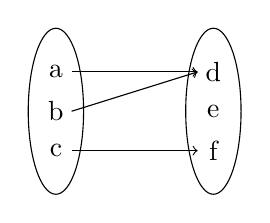
\begin{tikzpicture}
            \draw (0,0) ellipse (10pt and 30pt);
            \draw (2,0) ellipse (10pt and 30pt);

            \draw node at (0, 0.5) {a};
            \draw node at (0, 0) {b};
            \draw node at (0, -0.5) {c};

            \draw node at (2, 0.5) {d};
            \draw node at (2, 0) {e};
            \draw node at (2, -0.5) {f};

            \draw [->] (0 + 0.2, 0.5) -- (2 - 0.2, 0.5);
            \draw [->] (0 + 0.2, 0) -- (2 - 0.2, 0.5);
            \draw [->] (0 + 0.2, -0.5) -- (2 - 0.2, -0.5);
    \end{tikzpicture}
    \caption{Exemplo de função e seus conjuntos}
    \end{figure}

    \skipframe

    \item Na função abaixo, observe que:

    \begin{itemize}
        \item $D(f) = [-5, 3]$
        \item $Im(f) = [-2, 5]$
    \end{itemize}

    \begin{figure}
        \centering
        \begin{tikzpicture}[scale=0.6]
        \begin{axis}[xmin=-5, xmax=5, ymin=-5, ymax=5, axis lines=middle]
            \addplot[domain=-5:3]{x + 3};
        \end{axis}
        \end{tikzpicture}
        \caption{$f(x) = x + 3$}
    \end{figure}

    \skipframe

    \item Função: $f:\R \rightarrow \R \mid f(x) = x^2$:
    \begin{itemize}
        \item $D(f) = \R$
        \item $Im(f) = \R^+$
        \item $CD(f) = \R$
    \end{itemize}

    \begin{figure}
        \centering
        \begin{tikzpicture}[scale=0.6]
        \begin{axis}[xmin=-5, xmax=5, ymin=-5, ymax=5, axis lines=middle]
            \addplot{x^2};
        \end{axis}
        \end{tikzpicture}
        \caption{$f(x) = x^2$}
    \end{figure}

    \skipframe

    \item Função: $f:\R^+ \rightarrow \R \mid f(x) = \sqrt{x}$:
    \begin{itemize}
        \item $D(f) = \R^+$
        \item $Im(f) = \R^+$
        \item $CD(f) = \R$
    \end{itemize}

    \begin{figure}
        \centering
        \begin{tikzpicture}[scale=0.6]
        \begin{axis}[xmin=-5, xmax=5, ymin=-5, ymax=5, axis lines=middle]
            \addplot{sqrt(x)};
        \end{axis}
        \end{tikzpicture}
        \caption{$f(x) = \sqrt{x}$}
    \end{figure}

    \skipframe

    \item Função: $f:\R^* \rightarrow \R \mid f(x) = 1/x$:
    \begin{itemize}
        \item $D(f) = \R^*$
        \item $Im(f) = \R^*$
        \item $CD(f) = \R$
    \end{itemize}

    \begin{figure}
        \centering
        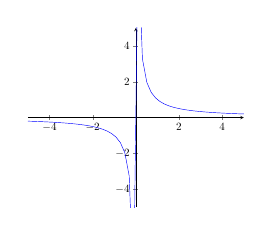
\begin{tikzpicture}[scale=0.4]
        \begin{axis}[xmin=-5, xmax=5, ymin=-5, ymax=5, axis lines=middle]
            \addplot[color=blue, samples=50]{1/x};
        \end{axis}
        \end{tikzpicture}
        \caption{$f(x) = 1/x$}
    \end{figure}

    
    
\end{itemize}
    
\end{frame}